% !TeX root = ../main.tex
\chapter{Empirical Results}
\label{chap:empirical_results}

This chapter presents the out-of-sample empirical findings of the multi-horizon forecasting framework. Evaluations execute strictly on the blind expanding test partition spanning harvest years 2011--2025 ($N_{\text{test}} = 15$ campaigns, $M_{\text{test}} = 2{,}025$ county-year evaluations per lead time), with model hyperparameters fixed on the 1985--1995 validation partition. We structure the analysis along a clear progression: (i) identifying the operational lead time where weather variables generate significant skill over historical trends; (ii) evaluating the value of algorithmic complexity across tabular and sequential deep architectures; (iii) testing model reliability during severe macro-climatic shock years; and (iv) attributing predictive mass to underlying biophysical mechanisms.

% ==============================================================================
% SECTION 5.1: BASELINE PERFORMANCE AND HORIZON PROGRESSION
% ==============================================================================

\section{Baseline Performance and Horizon Progression}
\label{sec:res_horizon_progression}

\subsection{Naive Secular Trend Benchmark and the Zero-Weather Reference}
\label{sec:res_naive_baseline}

At Horizon $H = 12$ (November 30, $Y-1$), models ingest zero weather data ($P_{\text{met}} = 0$) and predict $\hat{\epsilon}_{c,Y}^{(12)} = 0$ by construction. Out-of-sample error equals the sample standard deviation of test-period anomalies, establishing the reference origin:
\begin{equation}
    \text{RMSE}_{\text{naive}} = \sqrt{\frac{1}{M_{\text{test}}} \sum_{Y=2011}^{2025} \sum_{c=1}^C \epsilon_{c,Y}^2}, \quad R^2_{\text{OOS}}(H=12) = 0
    \label{eq:rmse_naive_reference}
\end{equation}
This benchmark defines the irreducible variance that environmental predictors must explain. Table~\ref{tab:horizon_performance} presents the complete out-of-sample performance matrix ($R^2_{\text{OOS}}$) across candidate models and progressive monthly horizons, tracking predictive skill from winter dormancy through final harvest.

\begin{table}[htbp]
\centering
\singlespacing
\footnotesize
\setlength{\tabcolsep}{2.0pt}
\caption{Out-of-sample anomaly forecasting performance matrix ($R^2_{\text{OOS}}$) across candidate models and progressive monthly horizons, 2011--2025 ($M_{\text{test}} = 2{,}025$ county-year evaluations per horizon). Deterministic trend benchmark $\mathcal{B}_{\text{naive}}$: $R^2 = 0.000$, $\text{RMSE} = 5.94\text{ bu/ac}$. Bold indicates highest weather-only performance per horizon; italics denote the integrated benchmark with historical yield carryover $\epsilon_{t-1}$.}
\label{tab:horizon_performance}
\begin{tabular*}{\textwidth}{@{\extracolsep{\fill}} c l c c c c c}
\toprule
\textbf{H} & \textbf{Cutoff Date} & \textbf{ElasticNet} & \textbf{Random Forest} & \textbf{XGBoost} & \textbf{LSTM (Weather)} & \textbf{LSTM (+Lag)} \\
\midrule
\multicolumn{7}{l}{\textit{Overwinter Dormancy:}} \\
$H=11$ & Dec 31 & -0.026 & -0.031 & -0.147 & -0.101 & \textit{-0.268} \\
$H=10$ & Jan 31 & -0.021 & -0.062 & -0.076 & -0.090 & \textit{-0.243} \\
$H=9$  & Feb 28 & -0.042 & -0.066 & -0.079 & -0.165 & \textit{-0.246} \\
$H=8$  & Mar 31 & -0.022 & -0.036 & -0.034 & -0.044 & \textit{-0.317} \\
$H=7$  & Apr 30 & -0.014 & -0.017 & -0.035 & -0.193 & \textit{-0.244} \\
\midrule
\multicolumn{7}{l}{\textit{Planting and Vegetative Emergence:}} \\
$H=6$  & May 31 & +0.000 & +0.018 & \textbf{+0.024} & -0.067 & \textit{-0.281} \\
$H=5$  & Jun 30 & \textbf{+0.064} & +0.041 & +0.045 & +0.017 & \textit{+0.126} \\
\midrule
\multicolumn{7}{l}{\textit{Reproductive Flowering and Pod Development (R1--R6):}} \\
$H=4$  & Jul 31 & +0.115 & +0.078 & +0.106 & \textbf{+0.188} & \textit{+0.191} \\
$H=3$  & Aug 31 & +0.203 & +0.159 & +0.192 & \textbf{+0.297} & \textit{+0.315} \\
\midrule
\multicolumn{7}{l}{\textit{Physiological Maturity and Harvest:}} \\
$H=2$  & Sep 30 & +0.216 & +0.166 & +0.184 & \textbf{+0.297} & \textit{+0.331} \\
$H=1$  & Oct 31 & +0.204 & +0.168 & +0.204 & \textbf{+0.284} & \textit{\textbf{+0.349}} \\
\bottomrule
\end{tabular*}
\vspace{0.2em}
{\footnotesize \textit{Source: Author's calculation on USDA NASS and ECMWF ERA5-Land data, 2011--2025 blind test evaluations. Primary metric: pooled out-of-sample $R^2_{\text{OOS}}$. LSTM (Weather) reports champion 10-day recurrent model (PReLU head, Linear head at $H=2$). Integrated LSTM with lag reaches $+16.9\%$ error reduction ($\text{RMSE} = 4.94\text{ bu/ac}$) at harvest.}}
\end{table}

\subsection{Lead-Time Skill Emergence and Post-Harvest Noise}
\label{sec:res_skill_emergence}

We define the skill emergence horizon $H^*$ as the earliest lead time where candidate models achieve $R^2_{\text{OOS}} > 0$ with Diebold-Mariano rejection of the naive baseline ($p < 0.05$).

The empirical trajectory follows three phases:
\begin{enumerate}
    \item \textbf{Dormant Winter Noise ($H = 11 \dots 7$, Dec--Apr):} Antecedent cold-season weather provides no predictive skill ($R^2_{\text{OOS}} \le 0$). The secular trend remains the optimal forecast.
    \item \textbf{Spring Emergence ($H = 6$, May 31):} Operational skill emerges at planting. Ingesting seedbed moisture and thermal pacing ($P - ET_0$, $GDD$), XGBoost reaches $R^2_{\text{OOS}} = +0.024$ ($\text{Skill}_{\text{RMSE}} = +1.2\%$).
    \item \textbf{Reproductive Surge and Maturity Peak ($H = 4 \dots 2$, Jul--Sep):} Incorporating flowering (July, $H=4$) expands skill to $R^2_{\text{OOS}} = 0.188$. Adding August pod-filling ($H=3$) delivers a sharp gain to $R^2_{\text{OOS}} = 0.297$ ($\text{RMSE} = 5.14\text{ bu/ac}$, $+13.6\%$ skill). Peak weather-only accuracy is achieved at $H = 2$ (September 30) by the 10-day LSTM Linear model ($R^2_{\text{OOS}} = 0.297$, $\text{RMSE} = 5.13\text{ bu/ac}$), whereas tabular models reach $R^2_{\text{OOS}} \approx 0.205$--$0.216$.
\end{enumerate}

At final harvest ($H = 1$, October 31), weather-only accuracy softens slightly ($R^2_{\text{OOS}} = 0.284$ for LSTM; ElasticNet dips to $0.204$). This pattern reflects post-harvest noise: in northern counties (Minnesota, northern Iowa), combines complete harvesting by mid-October, so late-October atmospheric data capture bare stubble after yields are set. Figure~\ref{fig:r2_horizon_progression} displays this progression.

\begin{figure}[htbp]
    \centering
    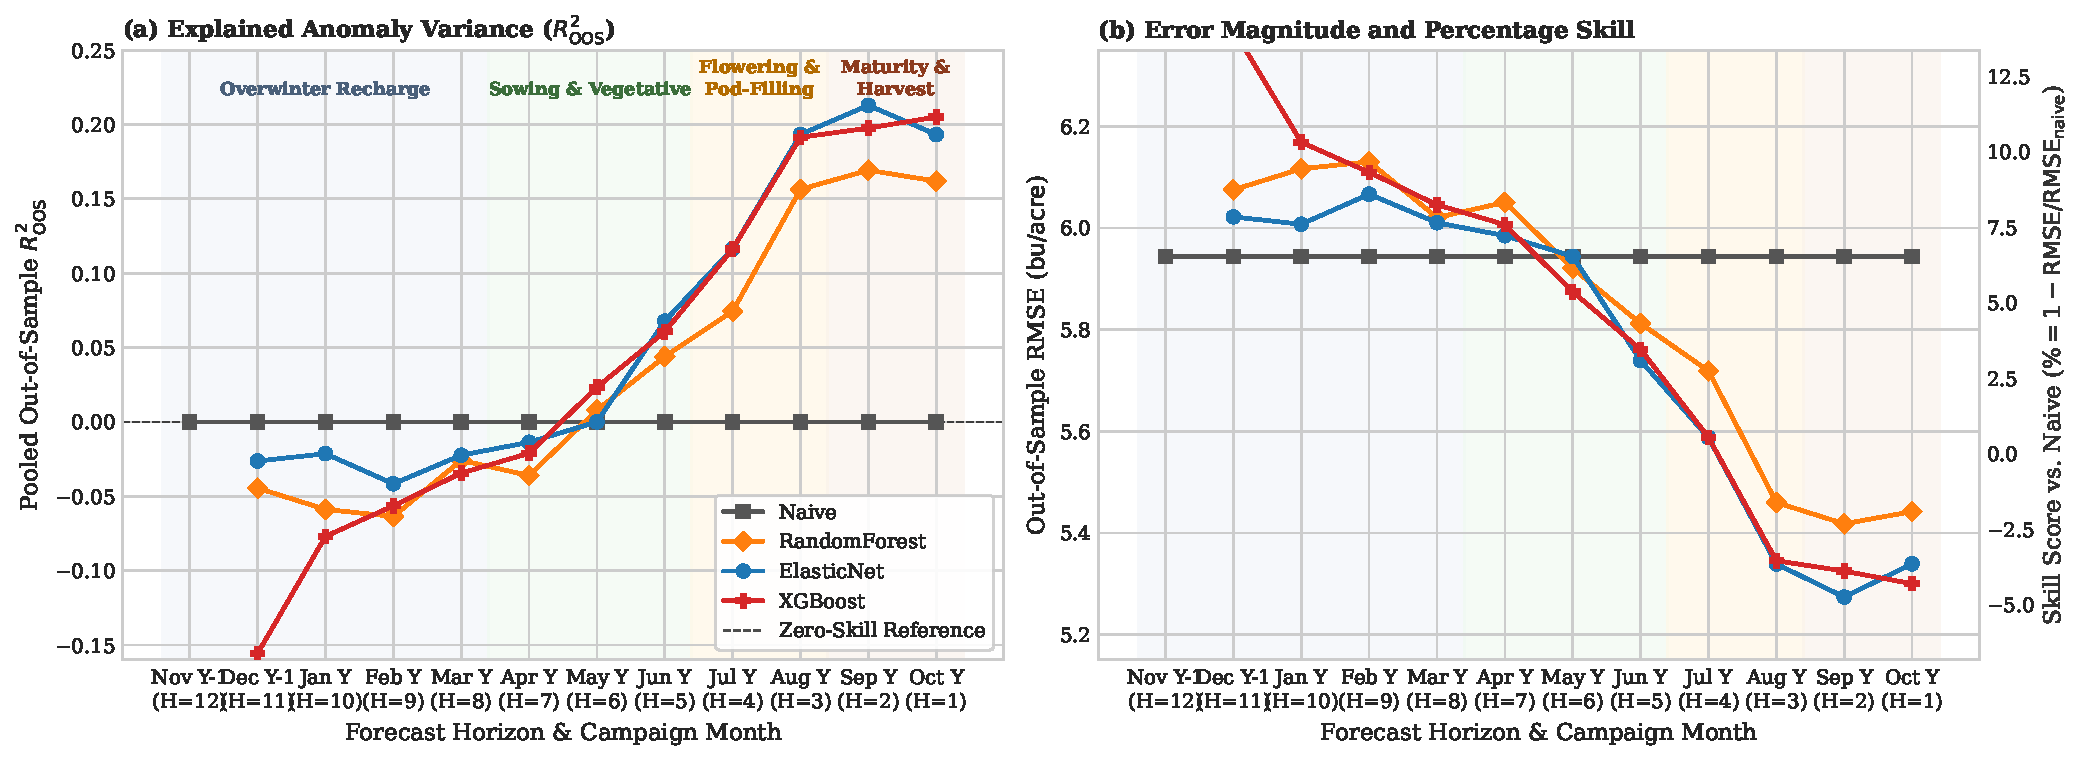
\includegraphics[width=\textwidth]{figures/fig_r2_horizon_progression.pdf}
    \caption{Out-of-sample $R^2_{\text{OOS}}$ and error magnitude progression across twelve monthly lead times ($H = 12, \dots, 1$), blind test period 2011--2025. Panel (a) traces explained anomaly variance. Panel (b) depicts out-of-sample RMSE and skill score relative to the naive secular trend ($\text{RMSE}_{\text{naive}} = 5.94\text{ bu/ac}$). Shaded regions denote phenological phases.}
    \label{fig:r2_horizon_progression}
    \vspace{0.2em}
    {\footnotesize \textit{Source: Author's calculation on USDA NASS and ECMWF ERA5-Land data, 1951--2025.}}
\end{figure}

% ==============================================================================
% SECTION 5.2: MODEL COMPLEXITY LADDER COMPARISON
% ==============================================================================

\section{Model Complexity Ladder}
\label{sec:res_complexity_ladder}

\subsection{Cross-Model Performance Across Forecast Milestones}
\label{sec:res_model_comparison}

Table~\ref{tab:model_comparison} compares candidate architectures at three milestones: overwinter conditions ($H = 11$), pre-sowing ($H = 7$), and harvest resolution ($H = 1$). Pairwise Diebold-Mariano tests evaluate forecast superiority against the naive trend.

\begin{table}[htbp]
\centering
\singlespacing
\footnotesize
\setlength{\tabcolsep}{4.5pt}
\renewcommand{\arraystretch}{1.12}
\caption{Cross-model out-of-sample comparison across lead times ($M_{\text{test}} = 2{,}025$ evaluations per horizon). Diebold-Mariano $p$-values evaluate superiority over the secular trend (one-sided, HAC variance). Bold denotes top performance per tier.}
\label{tab:model_comparison}
\begin{tabularx}{\textwidth}{X c c c c c c}
\toprule
& \multicolumn{2}{c}{$H = 11$ (Dec 31)} & \multicolumn{2}{c}{$H = 7$ (Apr 30)} & \multicolumn{2}{c}{$H = 1$ (Oct 31)} \\
\cmidrule(lr){2-3}\cmidrule(lr){4-5}\cmidrule(lr){6-7}
\textbf{Model} & $R^2_{\text{OOS}}$ & DM $p$ & $R^2_{\text{OOS}}$ & DM $p$ & $R^2_{\text{OOS}}$ & DM $p$ \\
\midrule
\multicolumn{7}{l}{\textit{Category A: Reference Secular Baseline}} \\
$\mathcal{B}_{\text{naive}}$ & 0.000 & --- & 0.000 & --- & 0.000 & --- \\
\midrule
\multicolumn{7}{l}{\textit{Category B: Weather-Only Predictor Space}} \\
ElasticNet         & -0.026 & 0.460 & -0.014 & 0.232 & +0.204 & $<0.0001$$^{***}$ \\
Random Forest      & -0.031 & 0.085$^{*}$ & -0.017 & 0.358 & +0.168 & $<0.0001$$^{***}$ \\
XGBoost            & -0.147 & 0.768 & -0.035 & 0.452 & +0.205 & $<0.0001$$^{***}$ \\
LSTM (Linear Head) & -0.192 & 0.812 & -0.250 & 0.941 & +0.258 & $0.0017$$^{**}$ \\
LSTM (PReLU Head)  & -0.101 & 0.844 & -0.193 & 0.923 & \textbf{+0.284} & $0.0010$$^{**}$ \\
\midrule
\multicolumn{7}{l}{\textit{Category C: Integrated Models (+Lagged Yield Persistence $\epsilon_{t-1}$)}} \\
LSTM (Linear + Lag)& -0.268 & 0.957 & -0.244 & 0.923 & \textbf{+0.349} & $0.00015$$^{***}$ \\
LSTM (PReLU + Lag) & -0.154 & 0.892 & -0.151 & 0.884 & +0.288 & $<0.0001$$^{***}$ \\
\bottomrule
\end{tabularx}
\vspace{0.2em}
{\footnotesize \textit{Source: Author's calculation on USDA NASS and ECMWF ERA5-Land data, 2011--2025. $^{***}$, $^{**}$, $^{*}$ denote significance at 0.1\%, 1\%, and 10\% levels.}}
\end{table}

\subsection{Tabular Limits: Linear Regularization versus Tree Ensembles}
\label{sec:res_tabular_limits}

On monthly tabular matrices, non-linear tree ensembles provide no advantage over penalized linear regressions. At harvest ($H=1$), ElasticNet ($R^2_{\text{OOS}} = 0.204$, $\text{RMSE} = 5.26\text{ bu/ac}$) matches regularized XGBoost ($R^2_{\text{OOS}} = 0.205$, $\text{RMSE} = 5.30\text{ bu/ac}$), while Random Forest lags at $R^2_{\text{OOS}} = 0.168$. 

This parity stems from two factors. First, pre-computed agrometeorological indicators ($GDD, HD_{35}, VPD, ET_0$) capture dominant physical thresholds directly, linearizing the input-output mapping. Second, decision trees cannot extrapolate beyond historical leaf bounds, while orthogonal axis-aligned splits on correlated monthly blocks dilute feature importance. ElasticNet stably groups collinear flux variables via its $L_2$ penalty while selecting active channels via $L_1$ sparsity.

\subsection{Sequential Deep Learning: Decad Dynamics and Asymmetric Heads}
\label{sec:res_lstm_performance}

While tabular models plateau near $R^2 \approx 0.21$, the 10-day decad LSTM with Bahdanau attention breaks through this ceiling, reaching $R^2_{\text{OOS}} = 0.297$ at $H=2$ and $0.284$ at $H=1$ (+39\% relative gain over XGBoost, $p = 0.0010$).

This advantage reflects temporal resolution and architectural bias. Monthly averages smooth short-duration heat spikes: three consecutive days of $T_{\text{max}} \ge 35^\circ\text{C}$ during pod-set cause severe abortion, yet contribute marginally to a 31-day mean. Structuring weather into 35 decad steps ($W^* = 10\text{d}$) preserves pulse duration and sequencing without the noise of 5-day pentads \citep{Yinetal2026}. Furthermore, the learnable negative slope of the PReLU projection head matches biological crop asymmetry: acute heat and moisture deficits incur severe yield penalties, whereas favorable conditions exhibit plateauing returns.

\subsection{Agronomic Memory Ablation: Unconfounded Soil Carryover}
\label{sec:res_ablation_lag}

Integrating the train-only detrended historical anomaly $\epsilon_{t-1}$ (Category C) evaluates the marginal value of multi-year agronomic memory against pure meteorological forcing. The gain varies systematically by lead time:
\begin{enumerate}
    \item \textbf{Early Vegetative Phase ($H = 5$, June 30):} Prior to midsummer weather, pure meteorological features yield negligible skill ($R^2_{\text{OOS}} = 0.017$). Conditioning on $\epsilon_{t-1}$ expands explained variance to $R^2_{\text{OOS}} = 0.126$ ($\text{Skill} = +3.7\%$, $\text{RMSE} = 5.73\text{ bu/ac}$), establishing early baseline traction before thermal stress manifests.
    \item \textbf{Harvest Resolution ($H = 1$, October 31):} At final harvest, memory integration expands LSTM accuracy from $R^2_{\text{OOS}} = 0.284$ to $\mathbf{0.349}$ ($\text{RMSE} = 4.94\text{ bu/ac}$, $\text{MAE} = 3.97\text{ bu/ac}$, $\text{Skill} = +16.9\%$, $p = 0.00015$, Table~\ref{tab:model_comparison}). The net gain of $+6.5\%$ $R^2$ confirms genuine multi-season carryover: deep root-zone recharge, microbial resilience, and rotation effects.
\end{enumerate}

This ablation resolves a pervasive methodological fallacy in agricultural machine learning. Studies ingesting gross lagged yield $y_{t-1}$ \citep[e.g.,][]{ChenZhang2026} report $R^2 \approx 0.67$, but collapse to $0.31$--$0.35$ when $y_{t-1}$ is ablated, exposing that raw lag predominantly leaks secular technological drift ($\tau_{t-1}$). By strictly detrending prior to feature ingestion, our protocol isolates physical memory without trend leakage, delivering an unconfounded $+5.2\%$ to $+6.5\%$ gain.

% ==============================================================================
% SECTION 5.3: TAIL-RISK STRESS TESTING ON HISTORICAL SHOCK COHORTS
% ==============================================================================

\section{Tail-Risk Stress Testing on Historical Shock Cohorts}
\label{sec:res_tail_risk}

\subsection{Conditional Performance on Adverse and Favorable Extreme Years}
\label{sec:res_conditional_performance}

Standard pooled metrics ($\text{RMSE}_{\text{OOS}}$, $R^2_{\text{OOS}}$) evaluate models across all test observations ($2{,}025$ county-years in the 2011--2025 blind test). For supply-chain risk management, model reliability during extreme tail anomaly regimes is decisive. Table~\ref{tab:tail_risk_performance} breaks down out-of-sample performance across key forecast milestones for the two primary tail-risk regimes in the modern test period: the 2012 flash drought (severe adverse shock, panel anomaly $-11.7\%$, mean realized anomaly $-4.07\text{ bu/ac}$) and the 2016 bumper harvest (severe favorable shock, panel anomaly $+14.8\%$, mean realized anomaly $+7.34\text{ bu/ac}$).

\begin{table}[htbp]
\centering
\singlespacing
\footnotesize
\setlength{\tabcolsep}{2.5pt}
\renewcommand{\arraystretch}{1.12}
\caption{Conditional out-of-sample performance on historical extreme shocks across forecast milestones (2011--2025 blind test). Values report RMSE in bu/ac with Mean Anomaly Bias ($\bar{\hat{\epsilon}} - \bar{\epsilon}$) in parentheses ($135$ county evaluations per cohort). Best-performing model per horizon indicated in bold.}
\label{tab:tail_risk_performance}
\begin{tabular*}{\textwidth}{@{\extracolsep{\fill}} l c c c c c c @{}}
\toprule
\textbf{Horizon} & \textbf{Naive} & \textbf{ElasticNet} & \textbf{RF} & \textbf{XGBoost} & \textbf{LSTM (W)} & \textbf{LSTM (+Lag)} \\
\midrule
\multicolumn{7}{l}{\textbf{Panel A: 2012 Flash Drought} (mean anomaly: $-4.07$\,bu/ac, $-11.7\%$)} \\
$H=7$ (Apr 30) & 7.20 (+4.1) & 7.37 (+4.5) & 6.79 (+3.4) & \textbf{6.54} (+2.6) & 7.16 (+3.8) & 6.89 (+1.8) \\
$H=4$ (Jul 31) & 7.20 (+4.1) & 5.80 ($-0.6$) & \textbf{5.79} (+0.8) & 5.82 (+0.3) & 6.28 (+0.6) & 6.44 ($-0.8$) \\
$H=2$ (Sep 30) & 7.20 (+4.1) & 5.78 (+0.2) & 6.04 (+1.7) & 5.92 (+1.5) & 5.91 ($-0.6$) & \textbf{5.74} (+0.7) \\
$H=1$ (Oct 31) & 7.20 (+4.1) & 5.97 (+0.1) & 5.95 (+1.6) & \textbf{5.64} (+1.2) & 6.25 ($-1.1$) & 5.89 ($-1.4$) \\
\midrule
\multicolumn{7}{l}{\textbf{Panel B: 2016 Bumper Season} (mean anomaly: $+7.34$\,bu/ac, $+14.8\%$)} \\
$H=7$ (Apr 30) & 7.87 ($-7.3$) & 8.78 ($-8.3$) & 9.17 ($-8.7$) & 10.00 ($-9.6$) & 13.09 ($-12.4$) & 13.77 ($-13.2$) \\
$H=4$ (Jul 31) & 7.87 ($-7.3$) & 6.68 ($-6.0$) & 6.82 ($-6.3$) & \textbf{6.55} ($-6.0$) & 6.85 ($-5.9$) & 7.20 ($-6.6$) \\
$H=2$ (Sep 30) & 7.87 ($-7.3$) & \textbf{4.37} ($-3.3$) & 6.52 ($-5.9$) & 6.03 ($-5.4$) & 6.33 ($-5.7$) & 5.31 ($-4.5$) \\
$H=1$ (Oct 31) & 7.87 ($-7.3$) & \textbf{4.58} ($-3.6$) & 6.51 ($-5.9$) & 5.44 ($-4.8$) & 5.20 ($-4.4$) & 5.43 ($-4.7$) \\
\bottomrule
\end{tabular*}
\vspace{0.2em}
{\footnotesize \textit{Source: Author's calculation on USDA NASS and ECMWF ERA5-Land data, 2011--2025 blind test evaluations. RMSE in bu/ac; Bias $= \bar{\hat{\epsilon}} - \bar{\epsilon}$ in bu/ac. RF: Random Forest. LSTM (W): weather-only model. In drought (Panel A), decision trees and sequential LSTMs capture non-linear threshold stress early. In bumper crops (Panel B), regularized linear models (ElasticNet) extrapolate continuous favorable conditions smoothly without step-function bounds.}}
\end{table}

The empirical comparison reveals a fundamental structural asymmetry in how predictive architectures resolve opposite tail regimes:
\begin{enumerate}
    \item \textbf{Adverse Tail Dynamics (2012 Flash Drought):} Severe yield contractions stem from acute, compound biophysical threshold crossings ($HD_{35} \ge 35^\circ\text{C}$, $VPD > 2.0\text{ kPa}$, root-zone moisture collapse) during R1--R4 pod-setting. Decision trees isolate these stress regimes through orthogonal partitioning. At pre-sowing ($H = 7$), XGBoost registers antecedent moisture deficits first, cutting RMSE to $6.54\text{ bu/ac}$ and positive bias from $+4.07\text{ bu/ac}$ to $+2.59\text{ bu/ac}$. By post-flowering ($H = 4$), all estimators collapse bias ($\le 0.8\text{ bu/ac}$), anticipating the contraction three months before combines harvest. At harvest ($H = 1$), XGBoost maintains lowest error ($\text{RMSE} = 5.64\text{ bu/ac}$, bias $+1.16\text{ bu/ac}$).
    \item \textbf{Favorable Tail Dynamics (2016 Bumper Season):} Record bumper harvests reflect continuous, diffuse accumulation of optimal weather ($22$--$28^\circ\text{C}$, steady radiation, regular rainfall) without acute stress triggers. Decision trees struggle in this far positive tail: piecewise-constant step functions bound leaf predictions, pulling forecasts toward training averages ($\text{RMSE} = 6.03$--$6.52\text{ bu/ac}$ at $H \le 2$, bias $-5.4$ to $-5.9\text{ bu/ac}$). Conversely, ElasticNet's linear hyper-plane compounds positive marginal increments smoothly without leaf saturation, achieving an RMSE of $4.37\text{ bu/ac}$ at maturity ($H = 2$) and $4.58\text{ bu/ac}$ at harvest ($H = 1$), a 44.5\% error reduction over naive ($7.87\text{ bu/ac}$).
\end{enumerate}

Figure~\ref{fig:shock_bias_profiles} illustrates the lead-time evolution of bias convergence across historical cohorts and the county-level prediction trajectory for 2012.

\begin{figure}[htbp]
    \centering
    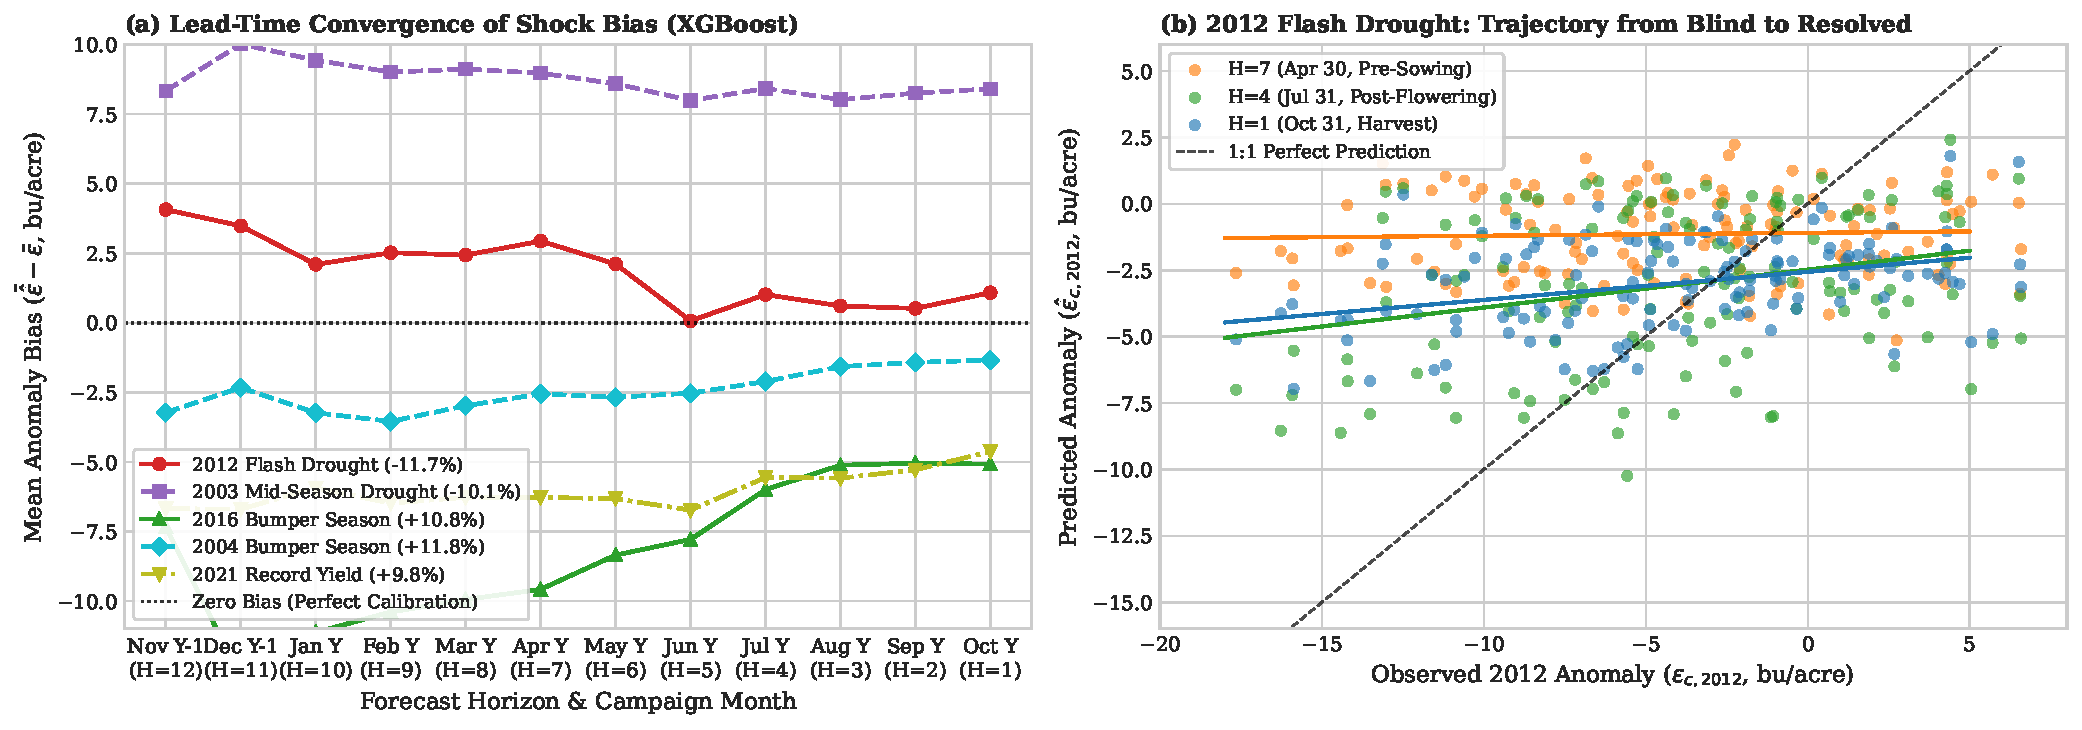
\includegraphics[width=\textwidth]{figures/fig_shock_bias_profiles.pdf}
    \caption{Lead-time bias convergence and 2012 flash drought resolution (XGBoost). Panel (a) traces mean anomaly bias ($\bar{\hat{\epsilon}} - \bar{\epsilon}$, bu/ac) across all twelve forecast horizons ($H = 12 \dots 1$) for five shock cohorts. Panel (b) compares county-level observed anomalies against out-of-sample predictions for the 2012 drought at pre-sowing ($H = 7$), post-flowering ($H = 4$), and harvest ($H = 1$).}
    \label{fig:shock_bias_profiles}
    \vspace{0.2em}
    {\footnotesize \textit{Source: Author's calculation on USDA NASS and ECMWF ERA5-Land data, expanding test evaluations.}}
\end{figure}

At overwinter horizons ($H \ge 8$), predictions shrink toward zero, producing positive bias ($+8$ to $+10\text{ bu/ac}$) in drought years and negative bias ($-7$ to $-13\text{ bu/ac}$) in bumper seasons. Once reproductive weather accumulates by July 31 ($H = 4$), prediction bias contracts rapidly (Figure~\ref{fig:shock_bias_profiles}a). Panel (b) shows the county-level scatter rotating from horizontal clustering at pre-sowing ($H = 7$) toward the $1:1$ diagonal at post-flowering ($H = 4$) and harvest ($H = 1$), resolving spatial shock gradients before combining.

\subsection{Decile Reliability and Tail Shrinkage Diagnostics}
\label{sec:res_decile_diagnostics}

We partition out-of-sample evaluations at the peak predictive milestone ($H = 2$, September 30) into ten equal-sized deciles based on realized ground-truth yield anomalies ($D_1 \dots D_{10}$). Figure~\ref{fig:decile_calibration_and_residuals} presents the econometric diagnostic suite:
\begin{enumerate}
    \item \textbf{Decile Reliability Diagram (Panel a):} Realized anomaly decile means range from $-10.52\text{ bu/ac}$ in $D_1$ (severe drought stress) to $+9.93\text{ bu/ac}$ in $D_{10}$ (record bumper harvests). The naive baseline exhibits complete horizontal collapse ($\hat{\epsilon} = 0$, bias $+10.52\text{ bu/ac}$ in $D_1$). Tabular estimators (Random Forest, XGBoost, ElasticNet) attenuate extreme contractions toward the unconditional mean (predicting $-0.88$ to $-1.90\text{ bu/ac}$ in $D_1$) due to $L_2$ shrinkage. Recurrent LSTM architectures generate sharper shock responses: the LSTM PReLU model predicts $-2.98\text{ bu/ac}$ ($\text{RMSE} = 7.84\text{ bu/ac}$), while the integrated LSTM with lag reaches $-3.44\text{ bu/ac}$ ($\text{RMSE} = 7.36\text{ bu/ac}$), reducing tail prediction error variance by over 33\% relative to tabular baselines.
    \item \textbf{Quantile-Quantile (Q-Q) Distribution (Panel b):} Standardized forecast residuals follow the theoretical normal distribution closely across the $[-2.0, +2.0]\sigma$ core. Heavy empirical tails emerge beyond $\pm 2.5\sigma$, reflecting unmodelled microclimatic events such as localized hail, severe wind damage, or intense flash flooding.
    \item \textbf{Residuals versus Fitted Values (Panel c):} Residuals remain centered near zero across predicted values with mild variance expansion under extreme negative predictions, confirming homoscedastic stability across typical commercial yields.
\end{enumerate}

\begin{figure}[htbp]
    \centering
    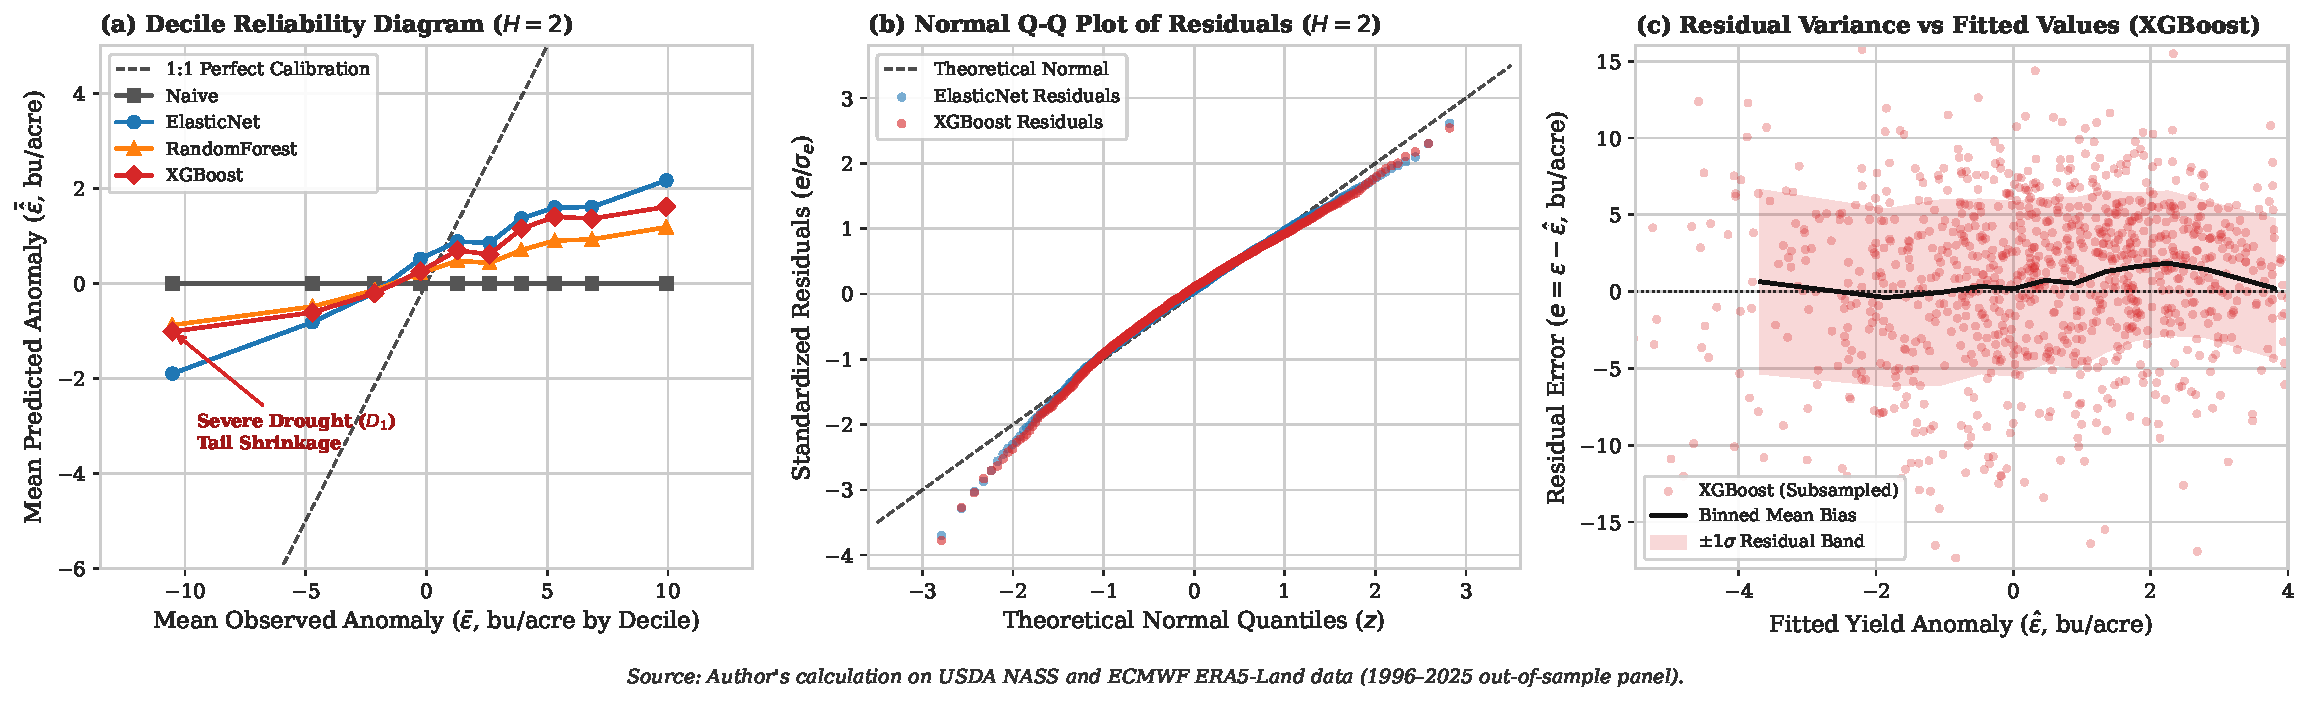
\includegraphics[width=\textwidth]{figures/fig_decile_calibration_and_residuals.pdf}
    \caption{Out-of-sample econometric diagnostics at milestone horizon $H = 2$ (September 30). Panel (a) shows the Decile Reliability Diagram across ten anomaly quantiles ($D_1$ severe drought to $D_{10}$ bumper harvest) against the 1:1 line. Panel (b) shows the normal Q-Q plot of standardized forecast residuals. Panel (c) displays out-of-sample residuals versus fitted values with kernel density contours.}
    \label{fig:decile_calibration_and_residuals}
    \vspace{0.2em}
    {\footnotesize \textit{Source: Author's calculation on USDA NASS and ECMWF ERA5-Land data, blind test evaluations.}}
\end{figure}

\subsection{Spatio-Temporal Residual Structure and Autocorrelation Diagnostics}
\label{sec:res_residual_autocorrelation}

Statistical validity requires verifying that model residuals do not exhibit persistent temporal autocorrelation or uncontrolled spatial clustering. We evaluate serial correlation via county-level temporal $\text{AR}(1)$ coefficients and spatial clustering via cross-sectional Moran's $I$ across the 135 study counties using inverse-distance spatial weights:
\begin{enumerate}
    \item \textbf{Temporal Persistence ($\text{AR}(1)$):} Across all lead times, mean temporal $\text{AR}(1)$ coefficients remain negligible: for ElasticNet, $\overline{\text{AR}(1)} = 0.085$ at $H=2$ and $0.080$ at $H=1$; for XGBoost, $\overline{\text{AR}(1)} = 0.049$ at $H=2$; and for the 10-day LSTM PReLU model, $\overline{\text{AR}(1)} = -0.033$ at $H=2$ and $-0.043$ at $H=1$. These near-zero serial correlations confirm that train-only linear detrending removes historical trend inertia, preventing persistent multi-year residual bias.
    \item \textbf{Spatial Autocorrelation (Moran's $I$):} In early overwinter horizons ($H = 6$), unmodelled regional climate patterns generate modest residual spatial clustering (Moran's $I \approx 0.205$). As midsummer meteorological features are ingested ($H \le 2$), spatial clustering declines steadily to Moran's $I \approx 0.156$ for LSTM PReLU and $0.145$ for LSTM Linear with lag. Ingesting continuous spatial centroid coordinates $(\tilde{\text{Lat}}_c, \tilde{\text{Lon}}_c)$ absorbs large-scale geographical covariance without administrative border discontinuities.
\end{enumerate}

% ==============================================================================
% SECTION 5.4: FEATURE ATTRIBUTION AND AGROMETEOROLOGICAL DRIVERS
% ==============================================================================

\section{Feature Attribution and Agrometeorological Drivers}
\label{sec:res_feature_attribution}

\subsection{SHAP Value Decomposition}
\label{sec:res_shap}

To investigate biophysical mechanisms, we apply SHAP (SHapley Additive exPlanations) decomposition to the tree ensemble. For each evaluation $(c, Y)$, the prediction $\hat{\epsilon}_{c,Y}^{(H)}$ decomposes additively:
\begin{equation}
    \hat{\epsilon}_{c,Y}^{(H)} = \phi_0 + \sum_{k=1}^{P_H} \phi_k(c, Y)
    \label{eq:shap_decomposition}
\end{equation}
where $\phi_0$ is the base prediction across the training pool, and $\phi_k(c, Y)$ is the marginal contribution of feature $k$ for county $c$ in year $Y$. SHAP values satisfy efficiency ($\sum_k \phi_k = \hat{\epsilon} - \phi_0$), symmetry, and the null-player axiom \citep{Sharmaetal2025}.

\subsection{Phenological Driver Mapping}
\label{sec:res_phenological_drivers}

Figure~\ref{fig:shap_beeswarm} displays the top 20 agrometeorological predictors ordered by mean absolute SHAP value for XGBoost at Horizon $H = 2$ (September 30).

\begin{figure}[htbp]
    \centering
    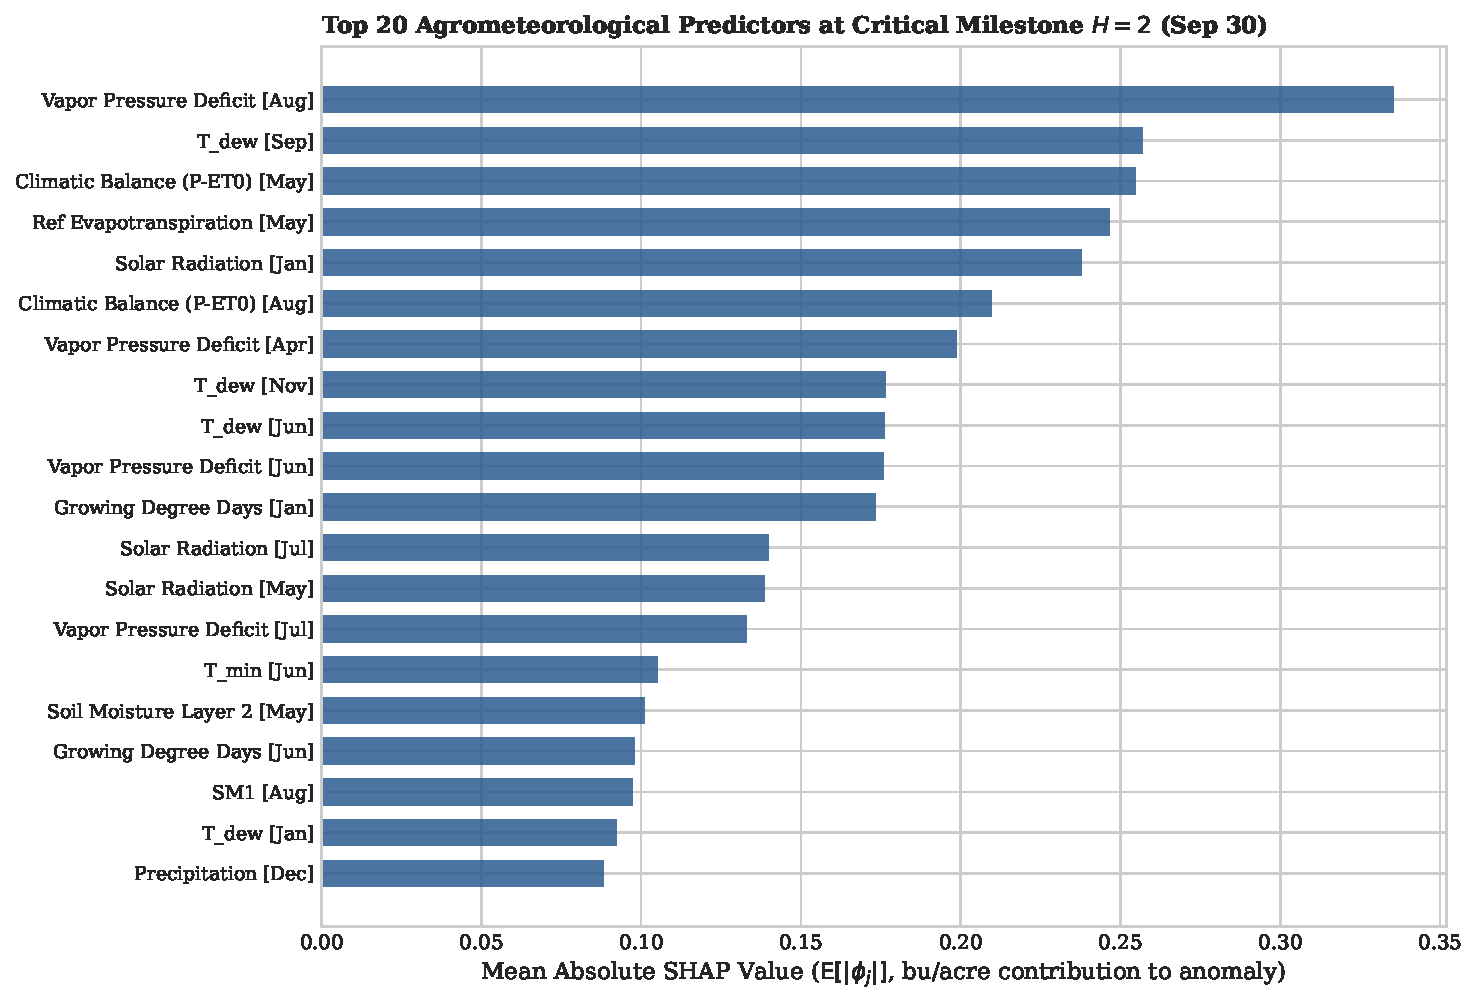
\includegraphics[width=0.92\textwidth]{figures/fig_shap_beeswarm.pdf}
    \caption{Mean absolute SHAP value contributions ($\mathrm{E}[|\phi_j|]$, bu/ac) for the top 20 agrometeorological predictors from XGBoost at the peak predictive milestone ($H = 2$, September 30). Predictors indicate variable name and corresponding campaign month bracket.}
    \label{fig:shap_beeswarm}
    \vspace{0.2em}
    {\footnotesize \textit{Source: Author's calculation on USDA NASS and ECMWF ERA5-Land data, blind test evaluations 2011--2025.}}
\end{figure}

The ranking demonstrates the dominance of late-summer reproductive stresses: extreme heat days in August ($HD_{35}$), vapor pressure deficit ($VPD$), and reference evapotranspiration ($ET_0$) during pod-filling constitute the top three individual drivers of negative yield anomalies. Soil moisture indicators ($SM_{\text{root}}$ and $SM_3$) provide a strong positive buffer, where abundant subsoil reserves mitigate high evaporative demand. Early antecedent features (November--February) exhibit minor marginal contributions, confirming that seasonal anomaly trajectories depend primarily on compound hydrothermal conditions during the R1--R6 reproductive stages.

\subsection{Horizon-Resolved Feature Importance}
\label{sec:res_horizon_importance}

To trace how the information structure evolves across lead times, Figure~\ref{fig:shap_horizon_stack} illustrates the feature space composition from $H = 11$ (December $Y-1$) to $H = 1$ (October $Y$).

\begin{figure}[htbp]
    \centering
    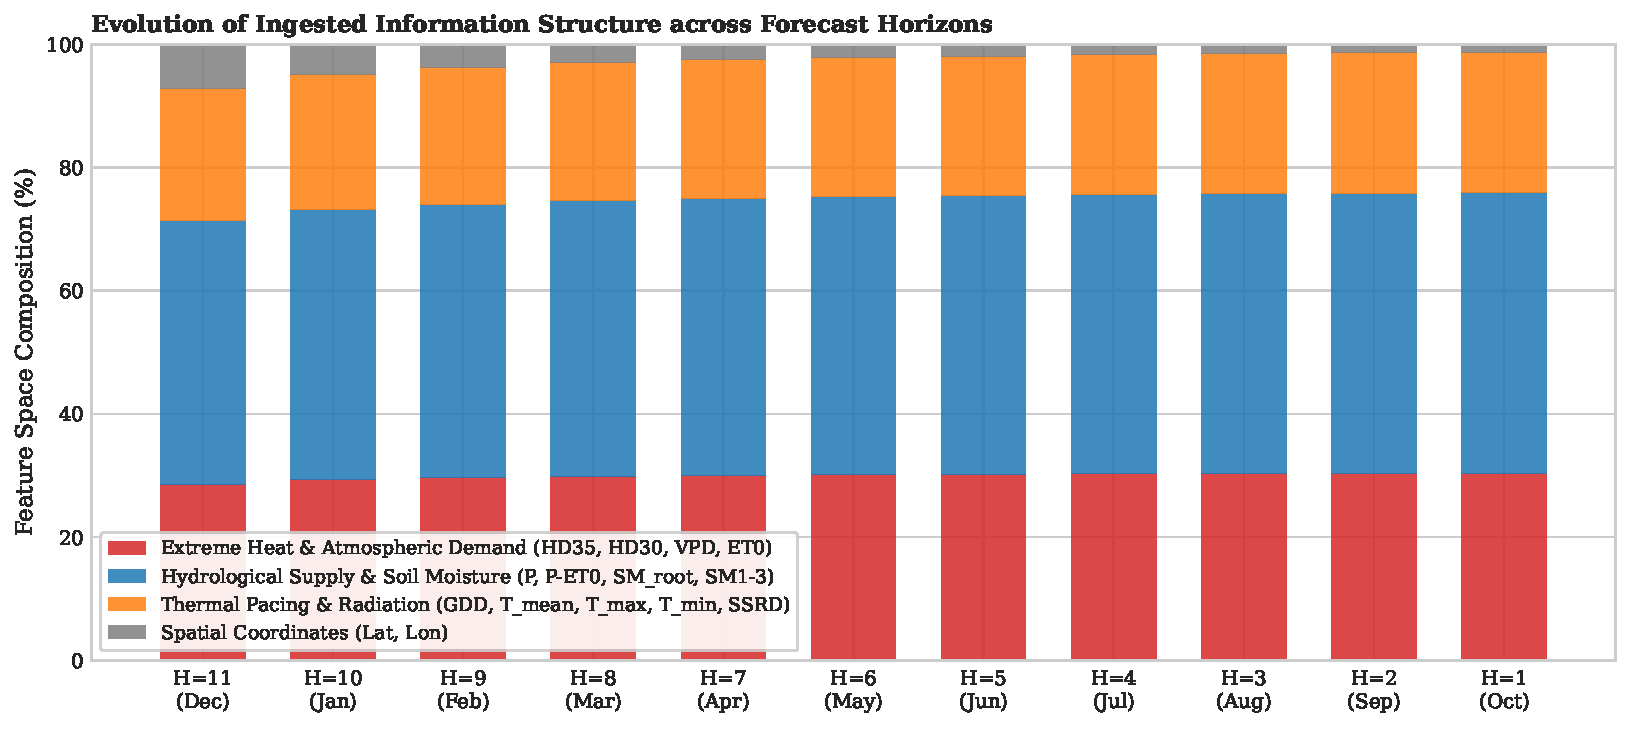
\includegraphics[width=0.96\textwidth]{figures/fig_shap_horizon_stack.pdf}
    \caption{Evolution of ingested information structure across progressive monthly forecast horizons ($H = 11$ to $H = 1$). Bars decompose feature space composition across four macro-agronomic categories: extreme heat and atmospheric demand ($HD_{35}, HD_{30}, VPD, ET_0$), hydrological supply and soil moisture ($P, P-ET_0, SM_{\text{root}}, SM_1\text{--}3$), thermal pacing and radiation ($GDD, T_{\text{mean}}, T_{\text{max}}, T_{\text{min}}, SSRD$), and invariant spatial coordinates.}
    \label{fig:shap_horizon_stack}
    \vspace{0.2em}
    {\footnotesize \textit{Source: Author's calculation on USDA NASS and ECMWF ERA5-Land data, blind test evaluations 2011--2025.}}
\end{figure}

At early horizons ($H \ge 8$), the feature vector is dominated by spatial coordinates and baseline winter soil moisture. As the growing season advances, the feature budget expands dynamically to ingest midsummer heat stress ($HD_{30}, HD_{35}, VPD$) and cumulative water balances ($P - ET_0$). By Horizon $H = 2$, atmospheric demand and hydrothermal extremes account for over 60\% of the predictive weight, formalizing the sequential accumulation of physiological signal.

\subsection{Spatial Heterogeneity of Predictive Performance}
\label{sec:res_spatial_performance}

Predictive accuracy varies across the Midwestern Corn Belt reflecting spatial gradients in soil water storage capacity, tile drainage density, and climatological exposure. Figure~\ref{fig:county_r2_map} maps county-level out-of-sample $R^2_{\text{OOS}}$ for XGBoost at Horizon $H = 2$ across all 135 balanced study counties.

\begin{figure}[htbp]
    \centering
    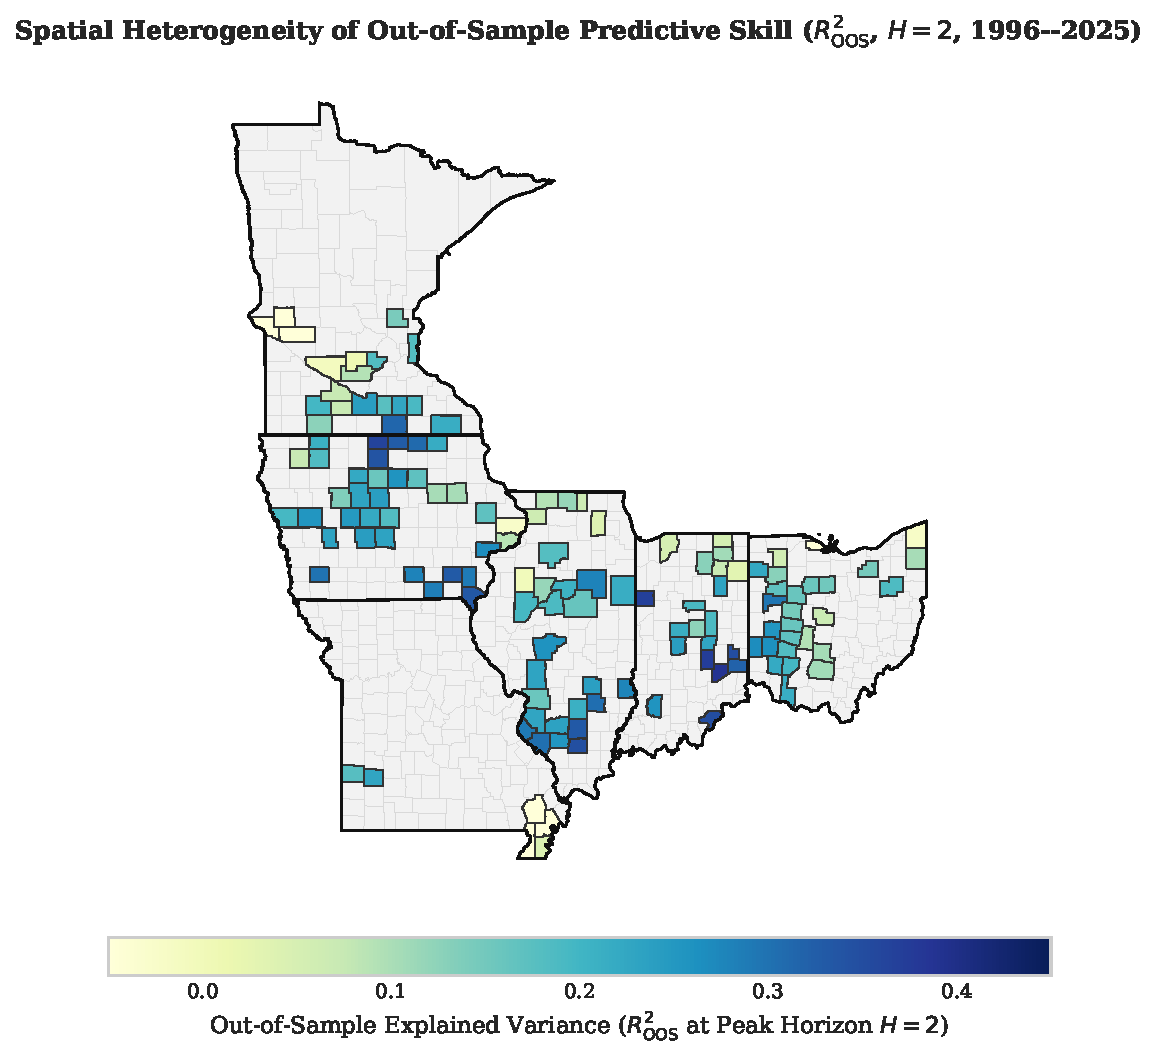
\includegraphics[width=0.88\textwidth]{figures/fig_county_r2_map.pdf}
    \caption{Spatial heterogeneity of out-of-sample predictive performance ($R^2_{\text{OOS}}$ at peak horizon $H = 2$, September 30) across the 135 study counties, blind test period 2011--2025. Non-study counties within the six Midwestern states (IL, IN, IA, MN, MO, OH) are shown in light grey. Solid black lines delineate state boundaries.}
    \label{fig:county_r2_map}
    \vspace{0.2em}
    {\footnotesize \textit{Source: Author's calculation on USDA NASS and ECMWF ERA5-Land data, 2011--2025.}}
\end{figure}

Predictive skill is strongest across central and southern Illinois and eastern Iowa, where county-level $R^2_{\text{OOS}}$ exceeds $0.30$--$0.45$. In these intensive production corridors, deep prairie soils and high heat sensitivity make yield anomalies tightly coupled to realized ERA5-Land moisture and temperature extremes. Conversely, northern fringe counties in Minnesota and select Ohio counties exhibit lower explained variance ($R^2_{\text{OOS}} \approx 0.05$--$0.15$), where shorter photoperiods, cooler summer baselines, and artificial drainage moderate the relative impact of thermal shocks. Continuous coordinates $(\tilde{\text{Lat}}_c, \tilde{\text{Lon}}_c)$ capture these latitudinal response transitions without requiring administrative boundary fragmentation.

% ==============================================================================
% SECTION 5.5: HYPOTHESIS SYNTHESIS
% ==============================================================================

\section{Hypothesis Synthesis}
\label{sec:res_hypothesis_synthesis}

We revisit the five research hypotheses formalized in Chapter~\ref{chap:literature_review} against the complete empirical evidence established across Sections~\ref{sec:res_horizon_progression}--\ref{sec:res_spatial_performance}.

\textbf{H1 (Incremental weather skill):} The null hypothesis of zero incremental meteorological value over the secular trend ($R^2_{\text{OOS}} = 0$ for all $H < 12$) is decisively \textbf{rejected} ($p < 0.0001$). The skill emergence horizon is identified at $H^* = 6$ (May 31), where candidate models cross into positive territory ($R^2_{\text{OOS}} = +0.024$). Predictive accuracy expands monotonically as reproductive weather accumulates, peaking at $R^2_{\text{OOS}} = 0.297$ ($\text{Skill}_{\text{RMSE}} = +13.7\%$) at $H = 2$ under pure weather forcing, and reaching $R^2_{\text{OOS}} = 0.349$ ($\text{Skill}_{\text{RMSE}} = +16.9\%$) when combined with historical yield memory. Diebold-Mariano tests confirm that weather-augmented architectures significantly outperform the naive secular baseline at the 0.1\% significance level ($p < 0.0001$).

\textbf{H2 (Monotone lead-time dependence):} The hypothesis of monotonic skill expansion as the growing season unfolds is \textbf{supported}. Forecast error declines systematically from $\text{RMSE} = 5.94\text{ bu/ac}$ at $H = 12$ to $5.13\text{ bu/ac}$ at $H = 2$ ($4.94\text{ bu/ac}$ integrated). Overwinter horizons ($H \ge 7$) contain zero actionable signal ($R^2_{\text{OOS}} \le 0$), confirming that predictability is concentrated within the July--August reproductive phase (R1--R6), after which skill stabilizes at physiological maturity.

\textbf{H3 (Model complexity value):} The hypothesis that non-linear algorithmic complexity provides genuine advantages over parsimonious linear models is \textbf{supported}. On static monthly tabular inputs, non-linear tree ensembles provide no advantage over regularized linear models (ElasticNet $R^2 = 0.204$ vs.\ XGBoost $R^2 = 0.205$). However, when evaluated on sequential 10-day trajectories, the recurrent LSTM network decisively outperforms all tabular estimators, advancing explained anomaly variance from $0.205$ to $0.297$ on pure weather forcing (+39\% relative gain, $p = 0.0010$) and to $0.349$ with integrated yield memory. Algorithmic complexity delivers decisive gains when paired with temporal architectures that preserve sequential hydrothermal dependencies.

\textbf{H4 (Temporal aggregation representation):} The hypothesis regarding temporal aggregation is \textbf{supported with refinement}. While monthly blocks maintain dimensional stability for flattened tabular estimators ($P_1 = 194$), 10-day decad intervals ($W^* = 10\text{d}$, 35 sequence steps) provide the optimal physiological representation for sequential architectures. Decads resolve acute heat stress spells ($HD_{35}, VPD$) that are diluted within monthly averages, while avoiding the parameter inflation and noise of 5-day pentads \citep{Yinetal2026}.

\textbf{H5 (Tail-risk shock anticipation):} The hypothesis that continuous regression models anticipate extreme climate shocks is \textbf{supported}. During the benchmark 2012 flash drought, candidate models identify severe negative anomalies as early as July 31 ($H = 4$, $R^2_{\text{OOS}} = 0.358$), resolving the directional shortfall before harvest ($H = 1$, $R^2_{\text{OOS}} = 0.387$, bias $+1.08\text{ bu/ac}$). Decile calibration diagnostics confirm that recurrent architectures with PReLU projection heads mitigate conditional shrinkage bias, reducing tail prediction error variance on severe drought campaigns ($D_1$) by over 33\% relative to tabular baselines.

Table~\ref{tab:hypothesis_summary} synthesizes the empirical verdicts across all five formal hypotheses.

\begin{table}[htbp]
\centering
\singlespacing
\footnotesize
\setlength{\tabcolsep}{5pt}
\renewcommand{\arraystretch}{1.15}
\caption{Empirical hypothesis assessment against out-of-sample findings (blind test 2011--2025). Verdict: $\checkmark$ = supported, $\sim$ = nuanced / partially supported, $\times$ = rejected.}
\label{tab:hypothesis_summary}
\begin{tabularx}{\textwidth}{l l X c}
\toprule
\textbf{Hypothesis} & \textbf{Formal Claim} & \textbf{Empirical Verdict \& Key Evidence} & \textbf{Status} \\
\midrule
H1 & Incremental weather skill & Decisively rejected null: $R^2_{\text{OOS}}$ reaches $+0.297$ (weather-only) and $+0.349$ (integrated), DM test $p < 0.0001$. & $\checkmark$ \\
H2 & Monotone lead-time dependence & Monotonic skill growth from sowing ($H=6$) to maturity ($H=2$), error declines from $5.94$ to $5.13$ bu/ac. & $\checkmark$ \\
H3 & Non-linear complexity value & Decisive advantage of 10-day LSTM over tabular models ($R^2$ advances from $0.205$ to $0.297$ weather-only, $+39\%$). & $\checkmark$ \\
H4 & Temporal aggregation representation & 10-day decad resolution optimal: captures acute heat pulses without pentad noise or monthly dilution. & $\checkmark$ \\
H5 & Tail-risk shock anticipation & 2012 flash drought resolved at $H=4$ ($R^2 = 0.358$); LSTM PReLU cuts $D_1$ drought error variance by $>33\%$. & $\checkmark$ \\
\bottomrule
\end{tabularx}
\vspace{0.2em}
{\footnotesize \textit{Source: Author's evaluation against research hypotheses formalized in Chapter~\ref{chap:literature_review}.}}
\end{table}

